\section{Auswertung}
\label{sec:Auswertung}
Aufgrund der zahlreichen Messwerte kann man die zeitlichen Temperaturverläufe sehr genau darstellen.
In den beiden folgenden Abbildungen sind die Temperaturunterschiede der äußeren Sensoren von Messing(breit)[T1], Messing(schmal)[T4] sowie Aluminium[T5] und Edelstahl[T8] gegenübergestellt.
% side-by-side Gegenüberstellung der ersten beiden plots
\begin{figure}
    \centering
    \begin{minipage}{.5\textwidth}
        \centering
        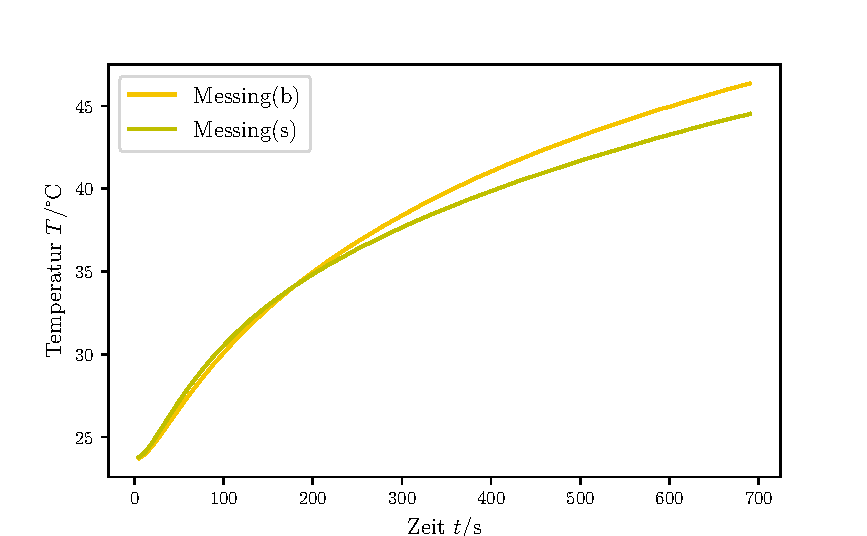
\includegraphics[max width=1.1\linewidth]{plots/plot_t1_t4.pdf}
        \caption{T1, T4}
        \label{fig:plot_t1_t4}
    \end{minipage}%
    \begin{minipage}{.5\textwidth}
        \centering
        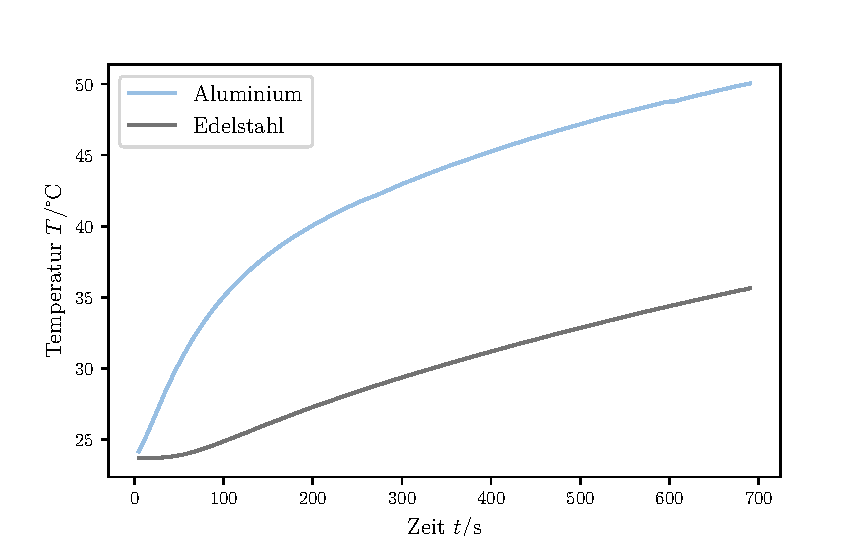
\includegraphics[max width=1.1\linewidth]{plots/plot_t5_t8.pdf}
        \caption{T5, T8}
        \label{fig:plot_t5_t8}
    \end{minipage}
    \caption{Zeitliche Temperaturverläufe außen}
    \label{fig:tempDiff_t1t4t5t8}
\end{figure}

\begin{table}
    \centering
    \caption{Temperatur außen nach 690 Sekunden in $\SI{}{\celsius}$}
    \label{tab:temp_aussen}
    \begin{tabular}{S[table-format=3.1, round-mode=places, round-precision=1] S[table-format=2.2] S[table-format=2.2] S[table-format=2.2] S[table-format=2.2]}
        \toprule
        {$t$} & {Messing(b)} & {Messing(s)} & {Aluminium} & {Edelstahl} \\
        \midrule
        690.0 & 46.36 &	44.53 &	50.04 &	35.64  \\
        \bottomrule
    \end{tabular}
\end{table}

$\symup{A}_{breit} = \SI{1.2}{\centi\m} \times \SI{0.4}{\centi\m} = \SI{0.48}{\square\centi\m}$

$\symup{A}_{schmal} = \SI{0.7}{\centi\m} \times \SI{0.4}{\centi\m} = \SI{0.28}{\square\centi\m}$ 

\begin{table}
    \centering
    \caption{Temperatur 5 verschiedener Messzeiten in $\si{\celsius}$}
    \label{tab:temp_5_messwerte}
    \begin{tabular}{S[table-format=3, round-mode=places, round-precision=1] S[table-format=2.2] S[table-format=2.2] S[table-format=2.2] S[table-format=2.2] S[table-format=2.2] S[table-format=2.2] S[table-format=2.2] S[table-format=2.2]}
        \toprule
        & \multicolumn{2}{c}{Messing(breit)} & \multicolumn{2}{c}{Messing(schmal)} & \multicolumn{2}{c}{Aluminium} & \multicolumn{2}{c}{Edelstahl} \\
        \cmidrule(lr){2-3}\cmidrule(lr){4-5}\cmidrule(lr){6-7}\cmidrule(lr){8-9}
        {$t[\si{\s}]$} & {$T_{1, \text{fern}}$} & {$T_{2, \text{nah}}$} & {$T_{3, \text{nah}}$} & {$T_{4, \text{fern}}$} & {$T_{5, \text{fern}}$} & {$T_{6, \text{nah}}$} & {$T_{7, \text{nah}}$} & {$T_{8, \text{fern}}$} \\
        \midrule
        60  & 27.45 &	31.68 &	32.57 &	27.94 &  31.50 & 34.49 & 29.59 & 24.03 \\
        150 & 32.77 &	36.49 &	36.83 &	32.97 &  38.00 & 40.03 & 34.40 & 26.11 \\
        295 & 38.24 &	41.41 &	40.97 &	37.54 &  42.83 & 44.47 & 38.19 & 29.27 \\
        475 & 42.69 &	45.63 &	44.63 &	41.26 &  46.73 & 48.27 & 41.70 & 32.46 \\
        640 & 45.61 &	48.52 &	47.26 &	43.85 &  49.33 & 50.89 & 44.27 & 34.95 \\
        \bottomrule
    \end{tabular}
\end{table}

\begin{table}
    \centering
    \caption{Temperaturunterschied nah zu fern in $\si{\celsius}$}
    \label{tab:tempdiff_5_messwerte}
    \begin{tabular}{S[table-format=3, round-mode=places, round-precision=1] S[table-format=1.2, round-mode=places, round-precision=2] S[table-format=1.2, round-mode=places, round-precision=2] S[table-format=1.2, round-mode=places, round-precision=2] S[table-format=1.2, round-mode=places, round-precision=2]}
        \toprule
        {$t[\si{\s}]$} & {$\increment T_{Messing(breit)}$} & {$\increment T_{Messing(schmal)}$} & {$\increment T_{Aluminium}$} & {$\increment T_{Edelstahl}$} \\
        \midrule
        60  & 4.23   & 4.6299 & 2.99 &	5.559 \\
        150 & 3.7199 & 3.8599 & 2.03 &	8.29 \\
        295 & 3.1699 & 3.4299 & 1.64 &	8.91 \\
        475 & 2.94   & 3.370  & 1.54 &	9.24 \\
        640 & 2.91   & 3.4099 & 1.56 &	9.32 \\
        \bottomrule
    \end{tabular}
\end{table}

\begin{equation}
    \frac{\increment \symup{Q}}{\increment \symup{t}} = -\kappa A \frac{\increment \symup{T}}{\increment \symup{x}}
\end{equation}

\begin{table}
    \centering
    \caption{Wärmestrom $\frac{\increment \symup{Q}}{\increment \symup{t}}$}
    \label{tab:Warmestrom}
    \begin{tabular}{l | S[round-mode=places, round-precision=4] S[round-mode=places, round-precision=4] S[round-mode=places, round-precision=4] S[round-mode=places, round-precision=4] S[round-mode=places, round-precision=4]}
        \toprule
        {Stoff} & {$\SI{60}{\s}$} & {$\SI{150}{\s}$} & {$\SI{295}{\s}$} & {$\SI{475}{\s}$} & {$\SI{640}{\s}$} \\
        \midrule
        Messing(breit)      & 0.758016    & 0.6666  & 0.56806 & 0.52684   & 0.52147   \\
        Messing(schmal)     & 0.483989  & 0.40349 & 0.358549 & 0.352277 & 0.35645 \\
        Aluminium           & 1.05726    & 0.71780   & 0.57990   & 0.54454   & 0.5516   \\
        Edelstahl           & 0.4092   & 0.61014  & 0.6565119 & 0.68006   & 0.68595   \\
        \bottomrule
    \end{tabular}
\end{table}

\begin{table}
    \centering
    \caption{Messreihe 2 - Dynamische Methode}
    \label{tab:data2}
    \begin{tabular}{S[table-format=3.1, round-mode=places, round-precision=1] S[table-format=2.2] S[table-format=2.2] S[table-format=2.2] S[table-format=2.2] S[table-format=2.2] S[table-format=2.2] S[table-format=2.2] S[table-format=2.2]}
        \toprule
        & \multicolumn{2}{c}{Messing(breit)} & \multicolumn{2}{c}{Messing(schmal)} & \multicolumn{2}{c}{Aluminium} & \multicolumn{2}{c}{Edelstahl} \\
        \cmidrule(lr){2-3}\cmidrule(lr){4-5}\cmidrule(lr){6-7}\cmidrule(lr){8-9}
        {$t$} & {$T_{1, \text{fern}}$} & {$T_{2, \text{nah}}$} & {$T_{3, \text{nah}}$} & {$T_{4, \text{fern}}$} & {$T_{5, \text{fern}}$} & {$T_{6, \text{nah}}$} & {$T_{7, \text{nah}}$} & {$T_{8, \text{fern}}$} \\
        \midrule
        0.000 & 33.08 &	36.21 &	36.46 &	32.47 &	34.62 &	37.16 &	33.62 &	29.54 \\
        0.500 & 33.10 &	36.25 &	36.48 &	32.50 &	34.66 &	37.19 &	33.65 &	29.55 \\
        1.000 & 33.12 &	36.27 &	36.51 &	32.52 &	34.69 &	37.25 &	33.68 &	29.54 \\
        $\vdots$ & $\vdots$ & $\vdots$ & $\vdots$ & $\vdots$ & $\vdots$ & $\vdots$ & $\vdots$ & $\vdots$ \\
        882.00 & 65.16 & 65.67 & 62.65 & 61.61 & 67.34 & 65.75 & 62.62 & 50.17 \\
        \bottomrule
    \end{tabular}
\end{table}

\begin{figure}
    \centering
    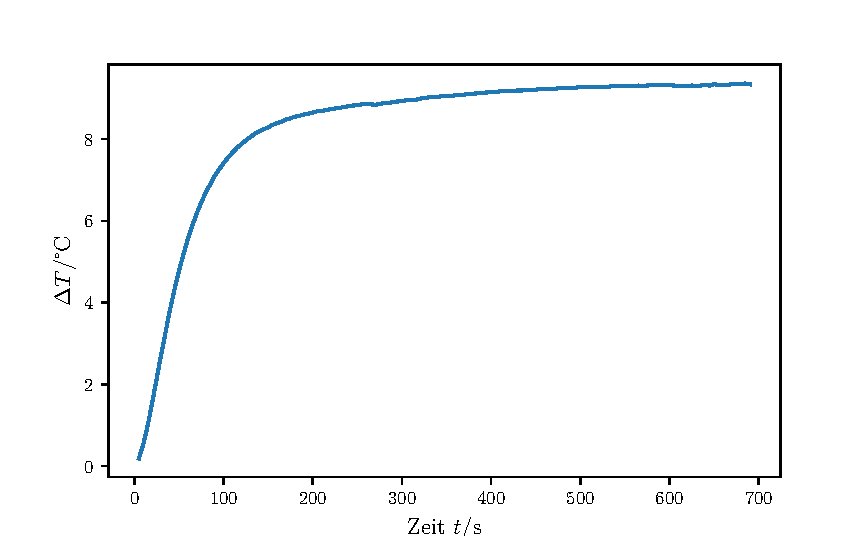
\includegraphics[max width=\linewidth]{plots/plot_tempDiff_steel.pdf}
    \caption{Erste Messung, statisch.}
    \label{fig:plot_tempDiff_t7t8}
\end{figure}

\begin{figure}
    \centering
    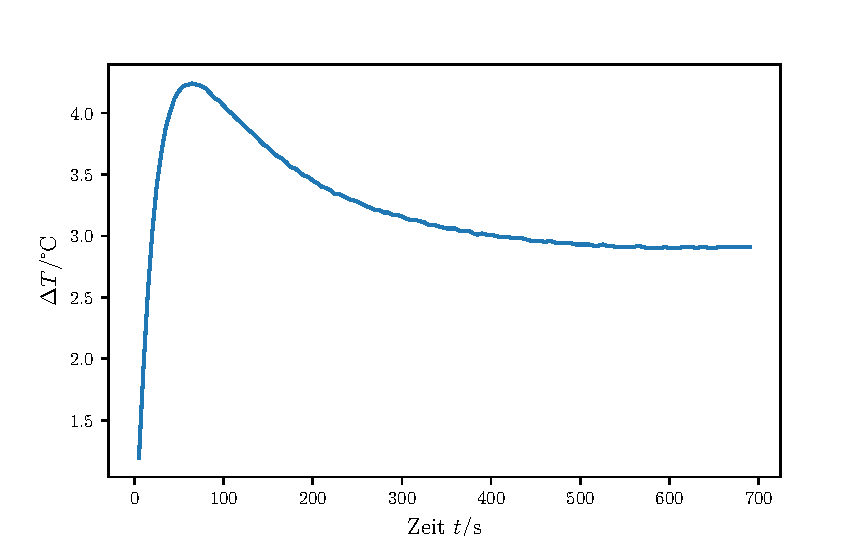
\includegraphics[max width=\linewidth]{plots/plot_tempDiff_brass_wide.pdf}
    \caption{Erste Messung, statisch.}
    \label{fig:plot_tempDiff_t2t1}
\end{figure}

% \begin{figure}
%     \centering
%     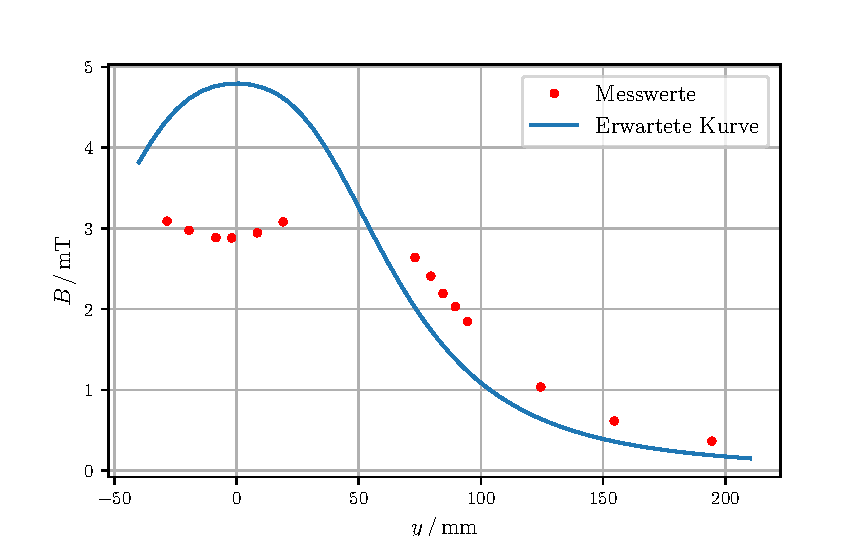
\includegraphics[max width=\linewidth]{plot2.pdf}
%     \caption{Zweite Messung, dynamisch.}
%     \label{fig:plot2}
% \end{figure}

% \begin{figure}
%     \centering
%     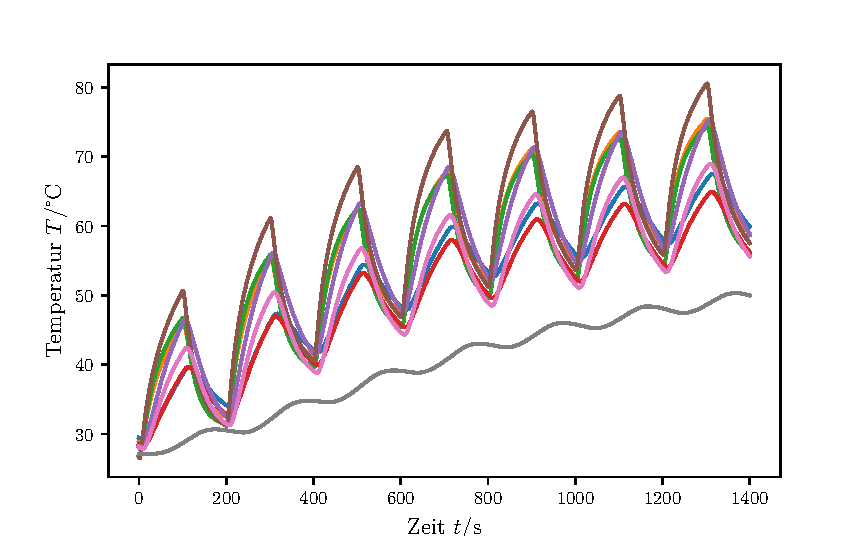
\includegraphics[max width=\linewidth]{plot3.pdf}
%     \caption{Dritte Mesuung, dynamisch - Angström.}
%     \label{fig:plot3}
% \end{figure}